\documentclass{article}
\usepackage{fancyhdr}
\usepackage{ctex}
\usepackage{listings}
\usepackage[a4paper, body={18cm,22cm}]{geometry}
\usepackage{amsmath,amssymb,amstext,wasysym,enumerate,graphicx}
\usepackage{float,abstract,booktabs,indentfirst,amsmath}
\usepackage{multirow}
\usepackage{enumitem}
\usepackage{listings}
\usepackage{xcolor}
\usepackage{tabularx}
\usepackage[most]{tcolorbox}
\usepackage{accsupp}
\usepackage[bottom]{footmisc}
\usepackage{subcaption}
% \usepackage[backend=biber,style=numeric]{biblatex}
\usepackage[xetex]{hyperref}
\usetikzlibrary{arrows.meta}
\newcommand\emptyaccsupp[1]{\BeginAccSupp{ActualText={}}#1\EndAccSupp{}}
\setlength{\parindent}{2em}
\renewcommand\arraystretch{1.4}
\setmonofont{Fira Code}
\setCJKmonofont{黑体}
% \setmainfont{Times New Roman}
\hypersetup{CJKbookmarks=true,colorlinks=true,citecolor=blue,%
            linkcolor=blue,urlcolor=blue,bookmarksnumbered=true,%
            bookmarksopen=true,breaklinks=true}
\lstset{
    % language = C,
    xleftmargin = 3em,xrightmargin = 3em, aboveskip = 1em,
	backgroundcolor = \color{white}, % 背景色
	basicstyle = \small\ttfamily, % 基本样式 + 小号字体
	rulesepcolor= \color{gray}, % 代码块边框颜色
	breaklines = true, % 代码过长则换行
	numbers = left, % 行号在左侧显示
	numberstyle = \small\emptyaccsupp, % 行号字体
    numbersep = -14pt, 
    keywordstyle=\color{purple}\bfseries, % 关键字颜色
    commentstyle =\color{red!50!green!50!blue!60}, % 注释颜色
    stringstyle = \color{red}, % 字符串颜色
    morekeywords={ASSERT, int64_t, uint32_t},
	frame = shadowbox, % 用(带影子效果)方框框住代码块
	showspaces = false, % 不显示空格
    showstringspaces = false,
	columns = fixed, % 字间距固定
    literate=
        {^+}{{{\color{black}\textbf{+}}\colorbox{green!30}{\phantom{XX}}}}1
        {+\t}{{{\color{black}\textbf{+}}\colorbox{green!30}{\phantom{XX}}}}1,
}

\raggedbottom

\title{\heiti\textbf{《软件测试与验证》课程论文解读报告}}
\author{L4-01: 王力 {\small 10225101434},武泽恺 {\small 10225101429},李鹏达 {\small 10225101460}}
\date{}

\newcommand{\flakyTest}{Flaky Test}

\begin{document}
\maketitle
\noindent \textbf{\heiti 论\qquad 文:}Do Automatic Test Generation Tools Generate Flaky Tests?\footnote{Martin Gruber, Muhammad Firhard Roslan, Owain Parry, Fabian Scharnböck, Phil McMinn, and Gordon Fraser. 2024. \textit{Do Automatic Test Generation Tools Generate Flaky Tests?} In Proceedings of the IEEE/ACM 46th International Conference on Software Engineering (ICSE '24). Association for Computing Machinery, New York, NY, USA, Article 47, 1–12. \url{https://doi.org/10.1145/3597503.3608138}}

\noindent \textbf{\heiti 实验仓库:}\small\url{https://doi.org/10.6084/m9.figshare.22344706.v3}

\section{背景介绍}
\textit{\flakyTest\footnote{Flaky Test暂时没有统一的中文翻译,因此在本报告中称英文原文}}是指在测试环境完全没有变化的情况下,有时通过有时失败的测试用例。\textit{Flakiness}是指\flakyTest 的如上所述的产生不稳定结果的特性。\flakyTest 的广泛存在,对软件开发者和研究者都构成了挑战。虽然针对开发者编写的\flakyTest 已有较多研究,但对于自动测试生成工具生成的\flakyTest 的研究较少。

\section{实验目标}

\begin{enumerate}[label=(\arabic*),noitemsep]
    \item 探究自动生成的测试中\flakyTest 的普遍性(Prevalence)。
    \item 验证EvoSuite的抑制\flakyTest 功能的有效性。
    \item 探究自动生成的\flakyTest 与开发者编写的\flakyTest 在根本原因上的差异。
\end{enumerate}

\section{实验过程}

\begin{figure}[htbp]
    \centering
    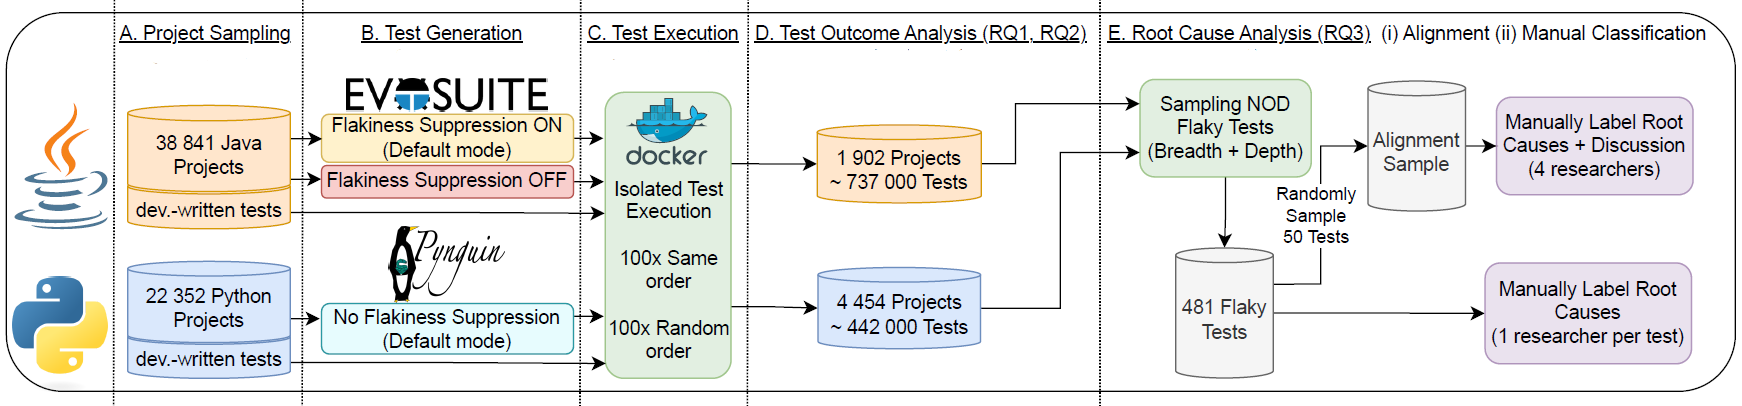
\includegraphics[width=\textwidth]{img/steps.png}
    \caption{实验过程}
    \label{fig:steps}
\end{figure}

图 \ref{fig:steps} 展示了实验的主要流程。

\subsection{工具选择}

\begin{itemize}
    \item 针对Java和Python两种语言,分别选择了EvoSuite和Pynguin两种流行的基于搜索的测试生成工具。
    \item 使用Flapy以在隔离的环境中执行测试并管理依赖。
\end{itemize}



\subsection{项目选择}

\begin{itemize}
    \item \textit{Java项目}:使用Maven中央仓库索引作为数据来源。限定选择的项目必须由Maven构建且源代码托管于GitHub上,最终筛选出38,841个项目。
    \item \textit{Python项目}:使用Python官方第三方软件仓库Python Package Index (PyPI)作为数据来源,随机抽取了22,352个项目。每个项目至少包含一个可以通过 pytest 执行的测试用例且项目源代码必须托管在 GitHub 上。
\end{itemize}

\subsection{测试生成}

\begin{itemize}
    \item \textit{Java项目}:EvoSuite有抑制\flakyTest 产生的机制,为了衡量这种机制的影响,实验采用EvoSuite${}_{FSOn}$(启用)和 \\
    EvoSuite${}_{FSOff}$(禁用)两种配置分别进行测试用例生成。测试生成范围则选择为每个项目的每个可测试类生成测试 ,可测试类的含义为至少包含一个公共方法的类。生成预算为每个可测试类设置2分钟的搜索时间。
    \item \textit{Python项目}:Pynguin没有可选的抑制Flakiness的参数,所以只在一种配置(默认配置)之下进行测试生成。生成范围为对每个项目中的每个模块生成测试。生成预算为每个模块10分钟的搜索时间。
\end{itemize}

EvoSuite和Pynguin生成测试具有不稳定性,每次运行可能生成不同的测试集。以往研究通常通过为每个项目生成多个测试集来应对这种随机性,而在此本研究中,对每个类(EvoSuite)或模块(Pynguin)仅生成一次测试集,以减少计算负担。为保证结果的普遍性,研究通过对大量项目进行抽样来弥补随机性的影响。

\subsection{测试执行}

为检测\flakyTest s,研究对开发者编写的测试和生成的测试分别执行200次,其中100次为固定顺序,100次为随机顺序。这是为了区分顺序依赖\flakyTest(OD)和非顺序依赖\flakyTest(NOD)。测试执行要么直接用FlaPy进行,要么仿照其原理进行,以确保每次测试执行都在一个隔离的环境中并管理依赖。开发者编写的测试和工具生成的测试分开运行,避免交叉影响。

对于项目的依赖安装,Java项目使用\texttt{mvn dependency:copy-dependencies}复制项目依赖。Python项目FlaPy 使用内置的依赖项安装功能。

对于随机顺序执行,Python项目通过pytest的“random-order”插件实现实现随机执行测试。Java由于Maven的Surefire插件不支持随机排序,研究团队开发了一个自定义测试运行器。

\subsection{测试输出结果分析}

\subsubsection{数据集分析}

作者计算了能够成功执行开发者编写的测试且能够在工具下生成测试的项目数量,这些项目是可以用于后续分析的数据集。
除此之外,为了确认是否获得了足够大且多样的项目集,实验采用了两项指标:
\begin{enumerate}[label=(\arabic*),noitemsep]
    \item 项目的源代码行数(LOC)
    \item 项目拥有的开发者编写的测试数量
\end{enumerate}
同时,为了确认实验是否正确使用了EvoSuite和Pynguin,作者还比较了自动生成测试的覆盖率和之前应用这些工具的研究所报告的覆盖率。

\subsubsection{普遍性}

为了研究\flakyTest 的普遍性,实验分析了

\begin{enumerate}[label=(\arabic*),noitemsep]
    \item 不使用 Flakiness 抑制机制的情况下生成的\flakyTest 数量与开发者编写的测试中发现的\flakyTest 数量。
    \item 顺序依赖\flakyTest (OD)与非顺序依赖\flakyTest (NOD)的比例。
    \item 至少包含一个开发者编写或工具生成的\flakyTest 的项目数量。
\end{enumerate}

\subsubsection{Flakiness抑制机制}

为了评估 EvoSuite的Flakiness抑制机制的效果,实验将
EvoSuite${}_{FSOn}$生成的\flakyTest 数量与EvoSuite${}_{FSOff}$生成的数量\flakyTest 数量以及开发者编写的\flakyTest 数量进行了比较。

\subsection{根本原因分析}

作者团队手动对\flakyTest 的根本原因进行标注。由于OD的\flakyTest 在随机顺序测试的步骤中能够被自动检测出,手动标注仅针对NOD的\flakyTest。按以下步骤进行检测:

\begin{enumerate}[label=(\arabic*),noitemsep]
    \item \textit{采样(Sampling)}:实验采用了广度采样和深度采样两种采样策略以保证样本的代表性。总计采样481个NOD \flakyTest 。其中329个来自广度采样,122个来自深度采样,30个同时被两种策略选中。
    
    \begin{itemize}[noitemsep]
        \item \textit{广度采样}:从每个受影响的项目中随机选择一个NOD \flakyTest,无论其类型是什么。
        \item \textit{深度采样}:随机选择21个Java项目和9个Python项目,采集这些项目中的所有NOD \flakyTest。这一步选择的项目包含的\flakyTest 均衡分布于不同类型。
    \end{itemize}

    \item \textit{标注(Labeling)}:四名作者根据项目代码、测试代码以及测试失败信息(如堆栈跟踪和错误消息)进行标注。为了确保作者们标注的一致性,作者们事先在50个\flakyTest 上分别独立进行了分类。然后作者们比对他们各自的结果,并对分歧进行了讨论整理,然后对根本原因类别做出了以下调整:
    
    \begin{itemize}[noitemsep]
        \item 将无序集合的类别拓宽,使其一般上也包括未指定的行为。
        \item 将类别“资源泄漏”的范围扩大,使其也涵盖资源不可用。
        \item 添加性能(category performance)类别,它描述了由于(连续)过程的持续时间 不同而间歇性失败的测试。
        \item 添加非幂等性结果(non-idempotent-outcome NIO)类别,涵盖了自污染和自状态设定测试。
    \end{itemize}

    \item \textit{基于标注的根本原因比较}:
    
    \begin{itemize}[noitemsep]
        \item 比较本研究中开发者编写测试的Flakiness根本原因与先前研究结果。
        \item 比较未启用Flakiness抑制机制的工具生成测试(EvoSuite${}_{FSOff}$、Pynguin)与开发者编写的测试的Flakiness根本原因。
        \item 比较启用(EvoSuite${}_{FSOn}$)与未启用(EvoSuite${}_{FSOff}$)Flakiness抑制机制的工具生成\flakyTest 的根本原因。
    \end{itemize}

\end{enumerate}

\subsection{有效性威胁分析}

作者从以下方面分析了对实验有效性的潜在威胁:

\begin{itemize}
    \item \textit{外部有效性(External Validity)}:外部有效性的威胁主要体现在项目的选取上。Java项目仅包括使用Maven的项目,并排除使用JUnit
    3的项目。Python项目基于现有数据集,该数据集已被多项研究使用,但可能继承其潜在缺陷。
    \item \textit{构建有效性(Construct Validity)}:首先,尽管实验顺序和乱序各执行了每个测试100次,但有的\flakyTest 发生概率较低,这将导致对\flakyTest 数量的低估。其次,为每个测试分配的生成预算是有限的,如果分配更多的时间可能会有不同的结果。
    \item \textit{内部有效性(Internal Validity)}:首先,因为实验产生的NOD \flakyTest 的数量过多而不得不采用抽样分析的方法,这个抽样过程对研究结果的有效性构成潜在威胁。其次,对\flakyTest 的根本原因标注由四位作者合作完成,因作者们对\flakyTest 的根本原因有不同的经验,这也导致了潜在的威胁。

\end{itemize}

\section{实验结果与分析}

\subsection{数据集分析}

\begin{figure}[htbp]
    \centering
    \begin{subfigure}[htbp]{0.45\textwidth}
        \centering
        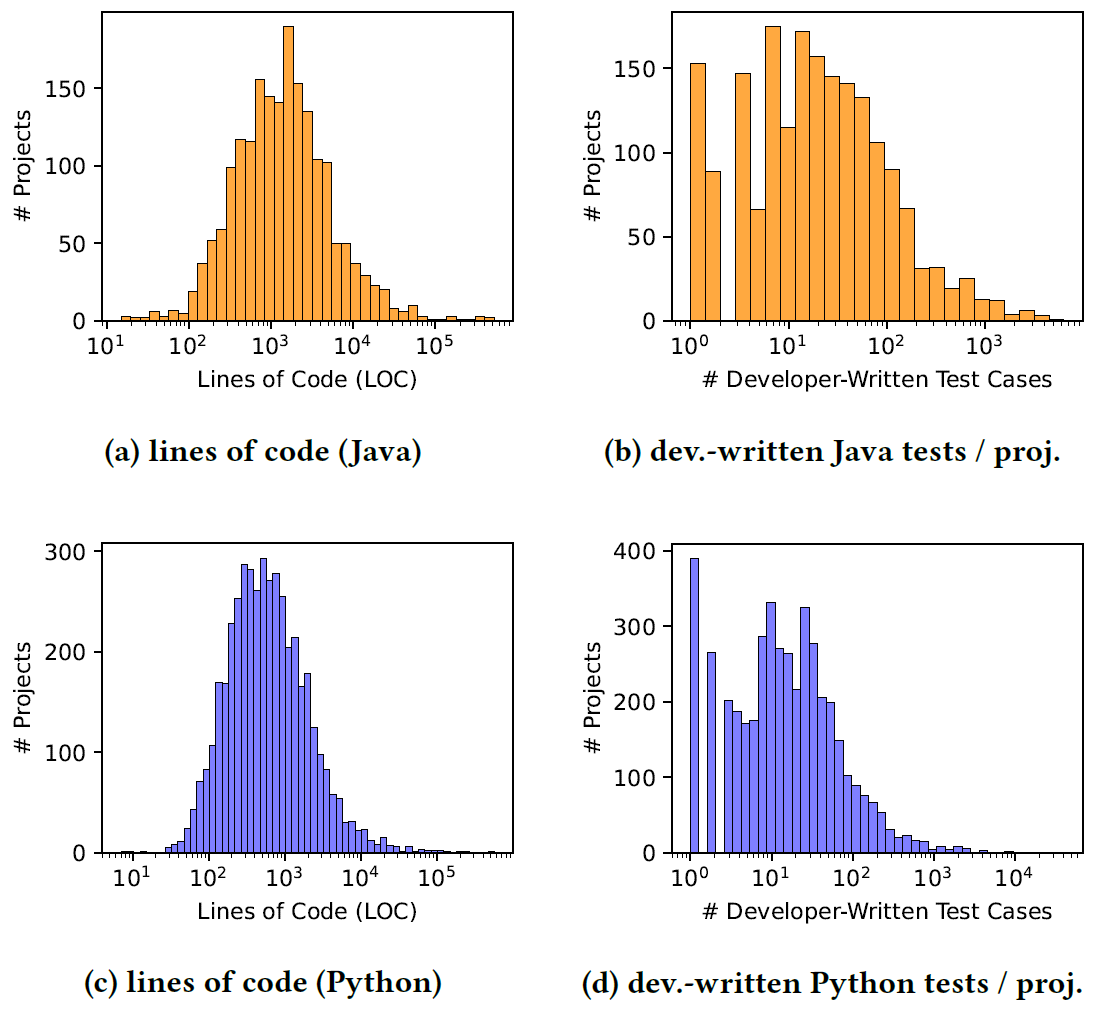
\includegraphics[width=\textwidth]{img/dataset.png}
    \end{subfigure}
    \begin{subfigure}[htbp]{0.45\textwidth}
        \centering
        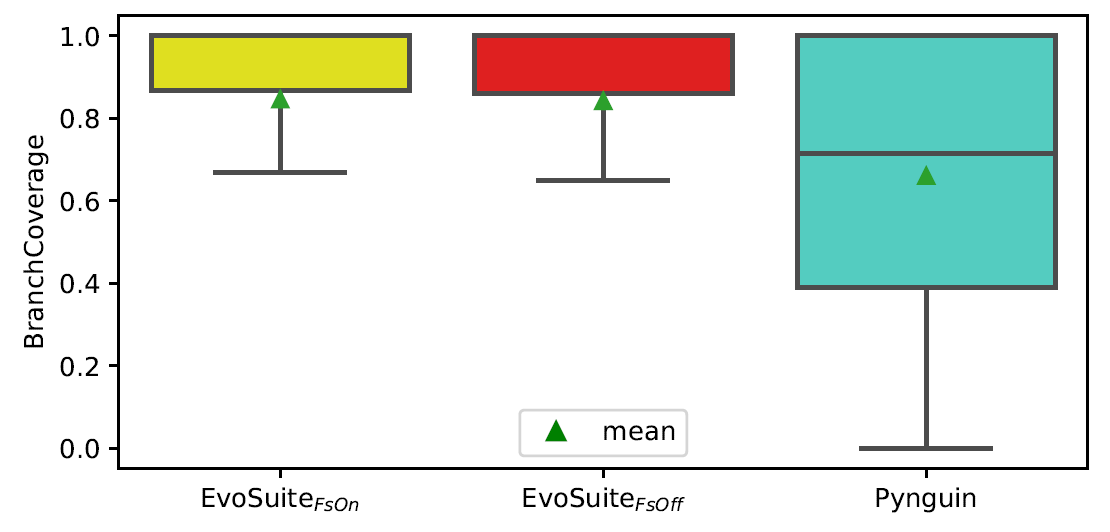
\includegraphics[width=\textwidth]{img/dataset_2.png}
    \end{subfigure}
    \caption{数据集分析}
    \label{fig:dataset}
\end{figure}

图 \ref{fig:dataset} 展示了有效数据集(能够成功执行开发者编写的测试且能够在工具下生成测试的项目)的统计信息。

\begin{itemize}
    \item \textit{Java项目}:代码平均行数为4,948,涵盖了从小于100行到大于50万行的范围。其中,共包含163,305个开发者编写用例,平均每个项目85.9个。EvoSuite生成测试覆盖率平均达81\%,与以往研究(84\%)相符。
    \item \textit{Python项目}:代码平均行数为1,755,涵盖了从小于100行到大于50万行。共包含303,711个开发者编写用例。平均每个项目68.2个。Pynguin生成测试覆盖率平均达66.0\%,与以往研究(71.6\%)非常接近。
\end{itemize}

这些结果表明,实验获得了足够大且多样的项目集,且实验正确使用了EvoSuite和Pynguin生成测试。

\subsection{自动化测试生成工具生成\flakyTest 的普遍性}

\begin{table}[htbp]
\centering
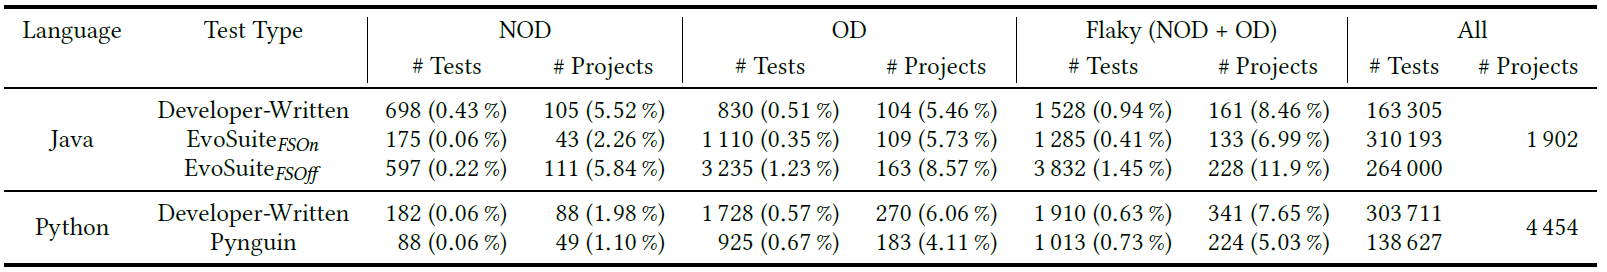
\includegraphics[width=\textwidth]{img/RQ1_res.png}
\caption{开发者编写的测试和自动生成的测试中\flakyTest 的数量}
\label{fig:rq1-res}
\end{table}

表 \ref{fig:rq1-res} 展示了开发者编写的测试和自动生成的测试中\flakyTest 的数量。在120万次测试中,共发现了9,568个\flakyTest ,其中约$2/3$的测试由自动化测试生成工具生成。

与开发者编写的测试相比,自动生成的测试更容易出现\flakyTest ,Java测试的比例增加了54\%(从0.94\%增加到1.45\%),Python测试的比例增加了16\%(从0.63\%增加到0.73\%),证实了\textbf{\flakyTest 在开发者编写和自动生成的测试中均普遍存在}。顺序依赖性方面,自动生成的Python测试与开发者编写的测试类似,顺序依赖性较强;而Java测试中开发者编写的测试表现均衡,自动生成的测试却更偏向顺序依赖性。

\begin{figure}[htbp]
\centering
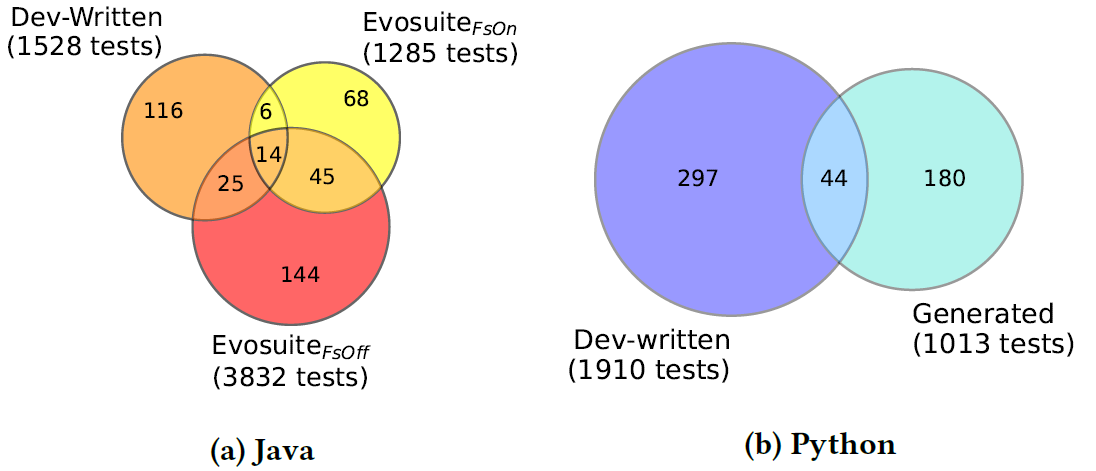
\includegraphics[width=0.5\textwidth]{img/RQ1_res2.png}
\caption{\flakyTest 的分布}
\label{fig:rq1-res2}
\end{figure}

图 \ref{fig:rq1-res2} 展示了\flakyTest 的分布,由自动化测试生成工具生成的\flakyTest 与开发者编写的测试交集较小,Java中仅有17.1\%的项目同时包含两类\flakyTest ,Python中为19.6\%。作者建议研究者可以进一步探索。

\subsection{自动化测试生成工具中Flakiness抑制机制的有效性}

如 表 \ref{fig:rq1-res} 所示,通过引入Flakiness抑制机制,\flakyTest 数量比例降低幅度达71.7\%(从1.45\%降至0.41\%),也远低于开发者手写测试的\flakyTest 数量比例(降低幅度达56.4\%),证实了\textbf{EvoSuite提供的Flakiness抑制机制能够有效降低测试的Flakiness}。同时,即使Flakiness抑制机制开启的情况下,仍然有86.4\%的flaky test表现出顺序依赖性。因此,作者不仅建议测试生成工具的维护者可以去借鉴EvoSuite的成功经验,也提议研究者对工具生成测试中的顺序依赖性进行进一步探讨。

\subsection{产生\flakyTest 的根本原因}
    
\begin{table}[H]
\centering
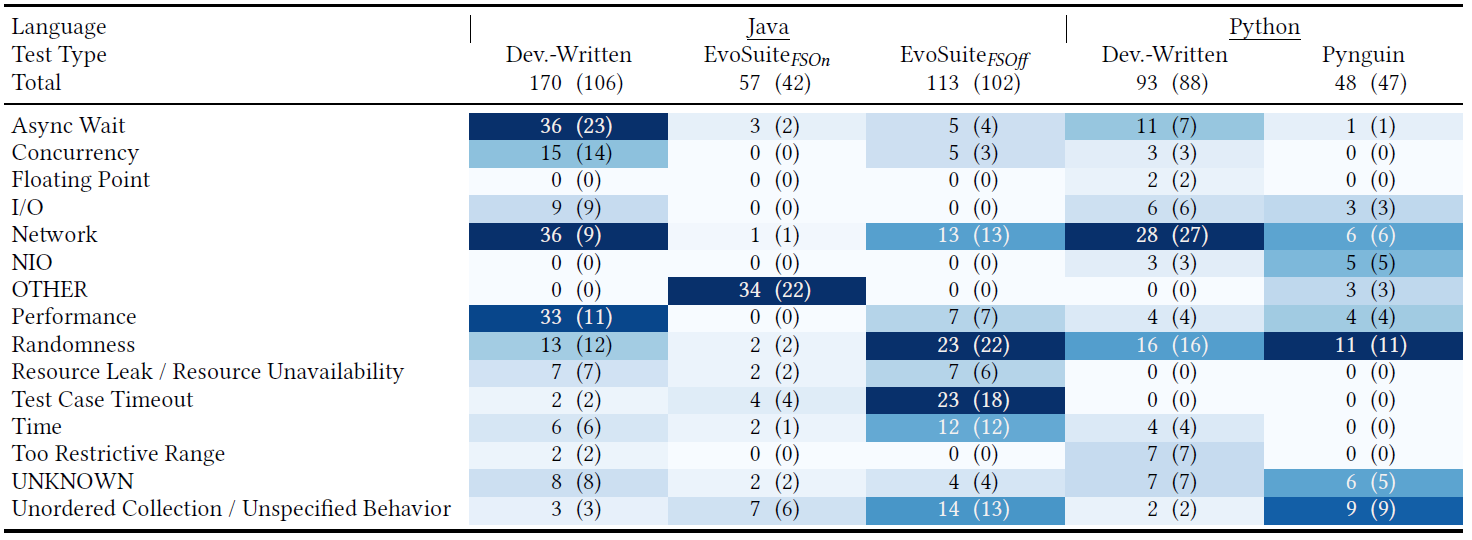
\includegraphics[width=\textwidth]{img/RQ3_res.png}
\caption{对于 NOD \flakyTest 根本原因的分析}
\label{fig:rq3-res}
\end{table}

表 \ref{fig:rq3-res} 展示了对于 NOD \flakyTest 根本原因的分析。
作者将\flakyTest 的根本原因归纳划分为15种。对于Java项目,开发人员编写的\flakyTest 的根本原因主要是异步等待(21.2\%)和性能假设(19.4\%),而Python项目主要由于网络(30.1\%)和随机性(17.2\%)问题。相比之下,未启用抑制机制所生成\flakyTest 主要由随机性(约20\%)和未指定的行为(12.4\%\textasciitilde18.7\%)导致;同时,EvoSuite生成的测试还会造成测试用例超时(20.4\%),而Pynguin生成的测试则会导致非幂等结果(10.4\%)。启用抑制机制后,传统根本原因(如随机性和超时)的\flakyTest 比例显著减少,但也引入了新类别问题,主要由运行时优化(如栈溢出错误等)和自动生成测试工具内部资源限制两类根本原因引起(59.6\%)。

结合分析,作者建议EvoSuite用户开启Flakiness抑制机制,并调整标志参数和移除特定脚手架文件,而Pynguin用户应设置随机数种子,从而尽可能地减少随机性带来的Flakiness。这些建议为目前部分已知根本原因的问题提供了有效解决方案。

\section{总结反思}

\flakyTest 是软件测试中常见且棘手的现象。在此研究中,研究团队证明了\flakyTest 在开发者编写的测试和软件生成的测试中均普遍存在,且 \flakyTest 在生成的测试中比在开发者编写的测试中更为常见。生成的测试与开发者编写的测试具有相同的根本原因,但这些原因的分布有所不同:开发者编写的\flakyTest 通常由并发和网络操作引起,而生成的\flakyTest 则往往是由随机性和未指定行为导致的。实验表明,EvoSuite的Flakiness抑制机制能够有效降低测试的Flakiness,但也可能会引入新类别的 \flakyTest——产生这些 \flakyTest 的根本原因与先前截然不同。 

此研究填补了现有研究中对自动生成测试中\flakyTest 的研究空白,并详细地分析了自动测试生成产生\flakyTest 的根本原因。研究结果为测试生成工具的维护者和研究者提供了有价值的见解。然而,我们认为以下问题仍然值得考虑:

\begin{enumerate}[label=(\arabic*),noitemsep]
    \item 研究只使用了EvoSuite和Pynguin两个工具,覆盖的语言仅限于Java和Python,限制了研究的普适性。实验结果显示,对于不同的语言和工具,\flakyTest 的根本原因可能会有所不同。\flakyTest 的产生的原因是否与语言本身特性有关?同一语言下,不同测试生成工具生成 \flakyTest 的根本原因是否相同?
    \item 研究虽然验证了EvoSuite的Flakiness抑制机制的有效性,但并未探究其具体原理。EvoSuite的Flakiness抑制机制是如何工作的?是否可以将这种机制应用到其他测试生成工具中?
    \item 研究中对于\flakyTest 的根本原因的分析是基于手动标注的,这可能会引入主观因素。是否可以通过机器学习等方法自动识别\flakyTest 的根本原因,以提高分析的准确性?
    \item 作者提供了实验的数据集、测试输出结果和分析测试输出结果的代码,但未提供生成和执行测试的代码,这使得读者难以重现实验的全部过程。
\end{enumerate}
\end{document}